% This file was created by matlab2tikz.
%
%The latest updates can be retrieved from
%  http://www.mathworks.com/matlabcentral/fileexchange/22022-matlab2tikz-matlab2tikz
%where you can also make suggestions and rate matlab2tikz.
%
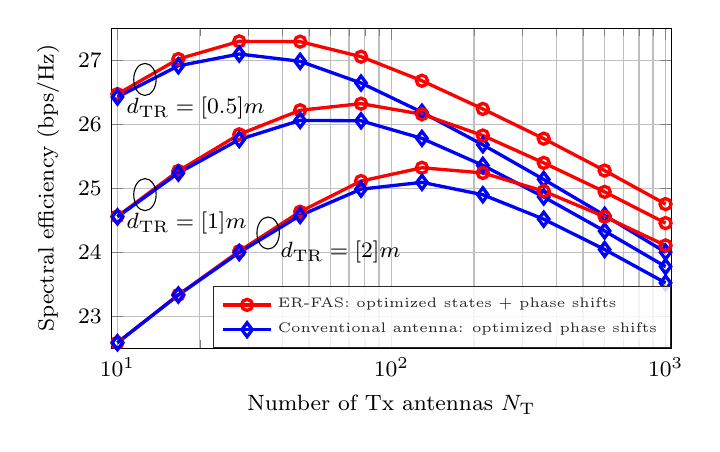
\begin{tikzpicture}[scale=1]

\begin{axis}[%
width=2.8in,
height=1.6in,
at={(0in,0in)},
scale only axis,
xmode=log,
xmin=9.5,
xmax=1050,
xminorticks=true,
xlabel style={font=\color{white!15!black},font=\footnotesize},
xticklabel style = {font=\color{white!15!black},font=\footnotesize},
xlabel={Number of Tx antennas $N_\mathrm{T}$},
ymin=22.5,
ymax=27.5,
ytick={23,24,25,26,27},
ylabel style={font=\color{white!15!black},font=\footnotesize},
yticklabel style = {font=\color{white!15!black},font=\footnotesize},
ylabel={Spectral efficiency (bps/Hz)},
axis background/.style={fill=white},
xmajorgrids,
xminorgrids,
ymajorgrids,
legend style={at={(1,0)}, anchor=south east, font=\tiny, legend cell align=left, align=left, draw=white!15!black, fill opacity=0.85}
]
\addplot [color=red, line width=1.2pt, mark=o, mark options={solid, red}]
  table[row sep=crcr]{%
10	26.4712074628579\\
16.6810053720006	27.0188465902714\\
27.8255940220712	27.2946548342627\\
46.4158883361278	27.2902027353343\\
77.4263682681127	27.0550905206984\\
129.154966501488	26.6795157626272\\
215.443469003188	26.2386358575941\\
359.381366380463	25.7745863196871\\
599.484250318941	25.2759800666057\\
1000	24.7519238723694\\
};
\addlegendentry{\ac{ER-FAS}: optimized states + phase shifts}

\addplot [color=blue, line width=1.2pt, mark=diamond, mark options={solid, blue},mark size=2.5pt]
  table[row sep=crcr]{%
10	26.4251410150594\\
16.6810053720006	26.9124107721767\\
27.8255940220712	27.0970919775509\\
46.4158883361278	26.9828989324395\\
77.4263682681127	26.64429843101\\
129.154966501488	26.1875711697996\\
215.443469003188	25.6789505164911\\
359.381366380463	25.1371679246426\\
599.484250318941	24.5762763069165\\
1000	24.0003295892389\\
};
\addlegendentry{Conventional antenna: optimized phase shifts}

\addplot [color=red, line width=1.2pt, mark=o, mark options={solid, red}, forget plot]
  table[row sep=crcr]{%
10	24.560080062499\\
16.6810053720006	25.2701020134103\\
27.8255940220712	25.841907369234\\
46.4158883361278	26.2182939609466\\
77.4263682681127	26.3212892938695\\
129.154966501488	26.1563148459005\\
215.443469003188	25.8234038481682\\
359.381366380463	25.3961151571643\\
599.484250318941	24.9432685699741\\
1000	24.454865847056\\
};
\addplot [color=blue, line width=1.2pt, mark=diamond, mark options={solid, blue},mark size=2.5pt, forget plot]
  table[row sep=crcr]{%
10	24.5525383673367\\
16.6810053720006	25.2372994123218\\
27.8255940220712	25.7610042831001\\
46.4158883361278	26.0599789064853\\
77.4263682681127	26.0538741709972\\
129.154966501488	25.7785896360876\\
215.443469003188	25.3572855787501\\
359.381366380463	24.8628301423659\\
599.484250318941	24.3311554317274\\
1000	23.7752113970412\\
};
\addplot [color=red, line width=1.2pt, mark=o, mark options={solid, red}, forget plot]
  table[row sep=crcr]{%
10	22.586611857715\\
16.6810053720006	23.3339937603806\\
27.8255940220712	24.0170144336728\\
46.4158883361278	24.6329027115887\\
77.4263682681127	25.1121095535015\\
129.154966501488	25.3198681829862\\
215.443469003188	25.2389899418525\\
359.381366380463	24.954298477285\\
599.484250318941	24.5546029105114\\
1000	24.1060924608517\\
};
\addplot [color=blue, line width=1.2pt, mark=diamond, mark options={solid, blue},mark size=2.5pt, forget plot]
  table[row sep=crcr]{%
10	22.586611857715\\
16.6810053720006	23.3308623927535\\
27.8255940220712	23.9957263179188\\
46.4158883361278	24.5738395506945\\
77.4263682681127	24.985570798367\\
129.154966501488	25.0917645631999\\
215.443469003188	24.8982024896258\\
359.381366380463	24.5165057649575\\
599.484250318941	24.0427476503587\\
1000	23.520955600272\\
};
\end{axis}

\begin{axis}[%
width=2.8in,
height=1.6in,
at={(0in,0in)},
scale only axis,
xmin=0,
xmax=100,
ymin=0,
ymax=100,
axis line style={draw=none},
ticks=none,
axis x line*=bottom,
axis y line*=left
  ]
  \draw [black] (axis cs:6,84) ellipse [x radius=2, y radius=5];
  \node[right, align=left]
    at (axis cs:1,75) {\footnotesize{$d_\mathrm{TR}=\unit[0.5]{m}$}};
  \draw [black] (axis cs:6,48) ellipse [x radius=2, y radius=5];
  \node[right, align=left]
    at (axis cs:1,39) {\footnotesize{$d_\mathrm{TR}=\unit[1]{m}$}};
  \draw [black] (axis cs:28,36) ellipse [x radius=2, y radius=5];
  \node[right, align=left]
    at (axis cs:28.5,30) {\footnotesize{$d_\mathrm{TR}=\unit[2]{m}$}};
  \end{axis}

\end{tikzpicture}%